\documentclass[14pt,a4paper]{scrartcl}
\usepackage{cmap}
\usepackage[utf8]{inputenc}
\usepackage[T1,T2A]{fontenc}
\usepackage[english,russian]{babel}
\usepackage{relsize}
\usepackage{graphicx}
\usepackage{subfigure}
\usepackage{mathtools}
\usepackage{amssymb}
\usepackage{float}
\usepackage{sidecap}
\usepackage{wrapfig}
\usepackage{caption}
\usepackage[table,xcdraw]{xcolor}
\usepackage{minted}
\begin{document}
	\begin{titlepage}
	\begin{center}
		\large
		МИНИСТЕРСТВО НАУКИ И ВЫСШЕГО ОБРАЗОВАНИЯ\\ РОССИЙСКОЙ ФЕДЕРАЦИИ
		
		\vspace{0.5cm}
		
		МГТУ им Н.Э.Баумана
		\vspace{0.25cm}
		
		Факультет ФН
		
		Кафедра вычислительной математики и математической физики
		\vfill
		
		
		Соколов Арсений Андреевич\\
		\vfill
		
		
		{\LARGE Часть 1 домашнего задания №2 \\ по теории случайных процессов\\[2mm]
		}
		\bigskip
		
		3 курс, группа ФН11-63Б\\
		Вариант 19
	\end{center}
	\vfill
	
	\newlength{\ML}
	\settowidth{\ML}{«\underline{\hspace{0.7cm}}» \underline{\hspace{2cm}}}
	\hfill\begin{minipage}{0.4\textwidth}
		Преподаватель\\
		\underline{\hspace{3cm}} Т.\,В.~Облакова\\
		«\underline{\hspace{0.7cm}}» \underline{\hspace{1.71cm}} 2019 г.
	\end{minipage}%
	\bigskip
	
	
	\vfill
	
	\begin{center}
		Москва, 2020 г.
	\end{center}
\end{titlepage}

\section*{Начальные данные}

Составим систему дифференциальных уравнений Колмогорова, отталкиваясь от размеченного графа $S$-однородного марковского процесса, предоставленного по условию:

\begin{figure}[H]
	\begin{minipage}[h]{1\linewidth}
		\center{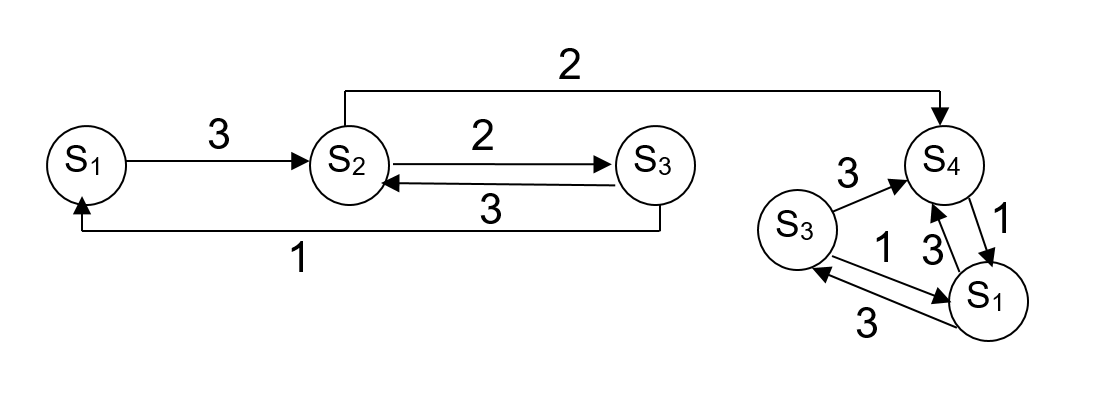
\includegraphics[width=1\linewidth]{../img/graph.png}}  \\
	\end{minipage}
\end{figure}

\begin{equation*}
\lambda = 
	\begin{pmatrix}
	0 & 0 & 1 & 1 \\
	3 & 0 & 3 & 0 \\
	3 & 2 & 0 & 0 \\
	3 & 2 & 3 & 0
	\end{pmatrix}
\end{equation*}
	
\begin{equation*}
	p(0) = (0 \; 1 \; 0 \; 0 \; 0)^T
\end{equation*}

Таким образом, вектор $p(t)$ вероятностей состояний изучаемой системы $S$ является решением следующей задачи Коши:

\begin{equation*}
	\begin{cases}
		p_1'(t) = p_3(t) + p_4(t);\\
		p_2'(t) = 3p_1(t) + 3p_3(t);\\
		p_3'(t) = 3p_1(t) + 2p_2(t);\\
		p_4'(t) = 3p_1(t) + 2p_2(t) + 3p_3(t);\\
		
		p_2(0) = 1;\\
		p_k(0) = 0, \qquad k = \{1,3,4,5\}.
	\end{cases}
\end{equation*}


Перепишем систему в изображениях:

\begin{equation*}
	\begin{cases}
		s\widetilde{p_1}(s) - p_1(0) = \widetilde{p_3}(s) + \widetilde{p_4}(t);\\
		s\widetilde{p_2}(s) - p_2(0) = 3\widetilde{p_1}(s) + 3\widetilde{p_3}(t);\\
		s\widetilde{p_3}(s) - p_3(0) = 3\widetilde{p_1}(s) + 2\widetilde{p_2}(t);\\
		s\widetilde{p_4}(s) - p_4(0) = 3\widetilde{p_1}(s) + 2\widetilde{p_2}(t) + 3\widetilde{p_3}(s);\\
		
		\widetilde{p_1}(s) + \widetilde{p_2}(s) + \widetilde{p_3}(s) + \widetilde{p_4}(s) = \frac{1}{s}.\\
	\end{cases}
\end{equation*}

Решая полученную систему, имеем:

\begin{equation*}
	\begin{cases}
		\widetilde{p_1}(s) = 
	\end{cases}
\end{equation*}



\end{document}